\section{fMRI analysis \label{multimodal:data:fMRI}}

Only the main characteristics of the fMRI analysis are described below; for a more detailed demonstration of fMRI analysis, read previous tutorial chapters describing fMRI analyses.

Toggle the modality from EEG to fMRI, and change directory to the fMRI subdirectory (either in \matlab\, or via the ``CD'' option in the SPM ``Utils'' menu)

\subsection{Preprocessing the fMRI data}

Press the \textsc{Batch} button and then:

\begin{itemize}
\item Select \textsc{Spatial: Realign: Estimate \& Reslice} from the SPM menu, create two sessions, and select the 390 \texttt{fM*.img} EPI images within the corresponding Session1 / Session 2 subdirectories (you can use the filter  \texttt{\textasciicircum fM.*}). In the ``Resliced images'' option, choose ``Mean Image Only''.

\item Add a \textsc{Spatial: Coreg: Estimate} module, and select the \texttt{smri.img} image in the \texttt{sMRI} directory for the ``Reference Image'' and select a ``Dependency'' for the ``Source Image'', which is the Mean image produced by the previous Realign module. For the ``Other Images'', select a ``Dependency'' which are the realigned images (two sessions) from Realign.

\item Add a \textsc{Spatial: Segment} module, and select the \texttt{smri.img} image as the ``Data''.

\item Add a \textsc{Spatial: Normalise: Write} module, make a ``New: Subject'', and for the ``Parameter File'', select a ``Dependency'' of the ``Norm Params Subj-$>$MNI'' (from the prior segmentation module). For the ``Images to Write'', select a ``Dependency'' of the ``Coreg: Estimate: Coregistered Images'' (which will be all the coregistered EPI images) and ``Segment: Bias Corr Images'' (which will be the bias-corrected structural image). Also, change the ``Voxel sizes'' to [3 3 3], to save diskspace.

\item Add a \textsc{Spatial: Smooth} module, and for ``Images to Smooth'', select a ``Dependency'' of ``Normalise: Write: Normalised Images (Subj 1)''.

\item Save the batch file (e.g, as \texttt{batch\_fmri\_preproc.mat}, and then press the ``Run'' button.
\end{itemize}

These steps will take a while, and SPM will output some postscript files with the movement parameters and the coregistration results (see earlier chapters for further explanation). The result will be a series of 2 sets of 390 \texttt{swf*.img} files that will be the data for the following 1st-level fMRI timeseries analysis.

\subsection{Statistical analysis of fMRI data}

First make a new directory for the stats output, e.g, a \texttt{Stats} subdirectory within the fMRI directory.

Press the \textsc{batch} button and then:

\begin{itemize}

\item Select ``Stats: fMRI model specification'' from the SPM module menu, and select the new \texttt{Stats} subdirectory as the ``Directory''.

\item Select ``Scans'' for ``Units of design''.

\item Enter \texttt{2} for the ``Interscan interval'' (i.e, a 2s TR).

\item Create a new session from the ``Data \& Design'' menu. For ``Scans'', select all the \texttt{swf*.img} files from the \texttt{Session1} subdirectory (except the mean). Under ``Multiple Conditions'', click ``Select File'', and select the \texttt{trials\_ses1.mat} file that is provided with these data. (This file just contains the onsets, durations and names of every event within each session.). For ``Multiple regressors'', click ``Select File'', and select the \texttt{rp*.txt} file that is also in the \texttt{Session1} subdirectory (created during realignment).

\item Repeat the above steps for the second session.

\item Under ``Basis Functions'', ''Canonical HRF'' add the ``Time and Dispersion'' derivatives.

\item Then add a ``Stats: Model estimation'' module, and for the ``Select SPM.mat'', choose the ``Dependency'' of the \texttt{SPM.mat} file from the previous ``fMRI model specification'' module.

\item Add a ``Stats: Contrast Manager'' module, and for the ``Select SPM.mat'', choose the ``Dependency'' of the \texttt{SPM.mat} file from the previous ``Model Estimation module''.

\item Under ``Contrast Sessions'', create a new F-contrast with a ``Name'' like \texttt{faces vs scrambled (all BFs)} and then enter  \texttt{[eye(3) -eye(3) zeros(3,6)]}. This will produce a 3x12 matrix that picks out the three basis functions per condition (each as a separate row), summing across the two conditions (with zeros for the movement parameter regressors, which are of no interest). Then select ``Replicate (average over sessions)''.

\item Under ``Contrast Sessions'', create a new F-contrast with a ``Name'' like \texttt{faces + scrambled vs Baseline (all BFs)} and then enter the \matlab \texttt{[eye(3) eye(3) zeros(3,6)]}. Again, select ``Replicate (average over sessions)''.

\item Save the batch file (e.g, as \texttt{batch\_fmri\_stats.mat}, and then press the ``Run'' button.

\end{itemize}

When this has finished, press \textsc{Results} and select the \texttt{SPM.mat} file that should have been created in the new \texttt{Stats} directory. The Contrast Manager window will appear, and you can select the ``faces vs scrambled (all BFs)'' contrast. Do not mask, keep the title, threshold at $p<.05$ FWE corrected, use an extent threshold of 60 voxels, and you should get the MIP and table of values (once you have pressed ``whole brain'') like that in Figure ~\ref{multimodal:fig:22}. This shows clusters in bilateral midfusiform (FFA), right occipital (OFA), right superior temporal gyrus/sulcus (STS), in addition to posterior cingulate and anterior medial prefrontal cortex. These clusters show a reliable difference in the evoked BOLD response to faces compared with scrambled faces that can be captured within the ``signal space'' spanned by the canonical HRF and its temporal and dispersion derivatives. Note that this F-contrast can include regions that show both increased and decreased amplitude of the fitted HRF for faces relative to scrambled faces (though if you plot the ``faces vs scrambled'' contrast estimates, you will see that the leftmost bar (canonical HRF) is positive for all the clusters, suggesting greater neural activity for faces than scrambled faces (also apparent if you plot the event-related responses)).

There is some agreement between these fMRI effects and the localisation of the differential ERP for faces vs scrambled faces in the EEG data (see earlier section). Note however that the fMRI BOLD response reflects the integrated neural activity over several seconds, so some of the BOLD differences could arise from neural differences outside the 0-600ms epoch localised in the EEG data (there are of course other reasons too for differences in the two localisations; see, eg, Henson et al, under revision).

\begin{figure}
\begin{center}
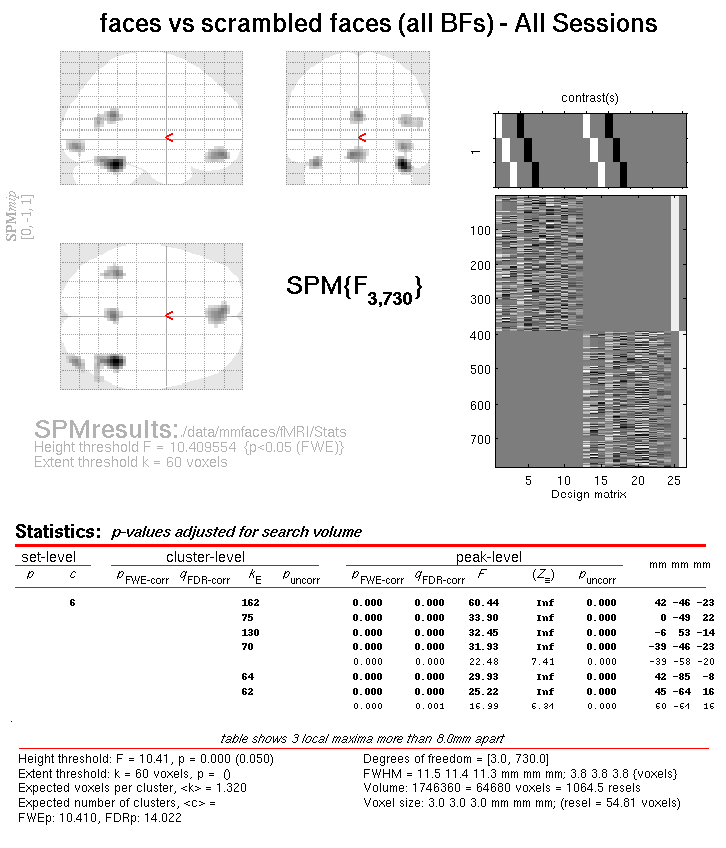
\includegraphics[width=150mm]{multimodal/figures/fmri_faces_vs_scrambled}
\caption{\em  SPM\{F\} for faces vs scrambled faces.\label{multimodal:fig:22}}
\end{center}
\end{figure}

You can also press \textsc{Results} and select the ``faces + scrambled vs Baseline (all BFs)'' contrast. Using the same threshold of $p<.05$ FWE corrected, you should see a large swathe of activity over most of the occipital, parietal and motor cortices, reflecting the general visuomotor requirements of the task (relative to interstimulus fixation). The more posterior ventral occipital/temporal BOLD responses are consistent with the MEG localisation of faces (or scrambled faces) versus baseline, though note that the more anterior ventral temporal activity in the MEG localisation is not present in the fMRI data, which suggests (but does not imply) that the MEG localisation may be erroneous.

These contrasts of fMRI data can now be used as spatial priors to aid the localisation of EEG and/or MEG data, as in the next section.
